\chapter{Introduction to Yaii Manual}

本书\footnote{本书标题及此章节标题特地不作翻译. }旨在告诉您, 如何快速高效地从互联网上获取信息, 以及如何避免来自广告、垃圾内容、恶意软件的骚扰. 

\section{入门章节}

\subsection{浏览器是您访问互联网的入口}

您的电脑桌面\footnote{入门章节提供的教程专门面向使用电脑设备的Windows用户, 如果您正在使用手机、平板等移动设备, 您可能需要适用于Android (安卓) 、iOS、iPadOS、鸿蒙系统的教程, 请参阅本手册后文的对应章节. }上可能有这样一个图标: 

\includegraphics[width=0.6in]{media/Internet_Explorer_4_and_5_logo.png}
\footnote{该Internet Explorer标志来源于 \url{https://commons.wikimedia.org/wiki/File:Internet_Explorer_4_and_5_logo.svg}, Credit by Microsoft, Public domain, via Wikimedia Commons}

它 (Internet
Explorer, IE浏览器) 是微软开发的一款网页浏览器, 它很旧, 即便是IE11也已经结束了它的生命周期\footnote{这意味着您永远都不会接收到关于它的更新了. 但是最主要的一点是随操作系统附带的IE版本太旧, 无法支持比较新的TLS标准, 这会导致您访问一些网站时被提示安全证书无效. }. 

为了访问现代网页\footnote{这通常是指由W3C制订的HTML5标准, 即现在最流行的网页呈现格式, 您所看到的网页还会一同使用CSS3标准、EMCA Script 6或者更新的标准. }, 您需要一个比较新的浏览器. \footnote{Windows 10/11的用户可能会使用系统附带的Edge浏览器, 如果您这么做了, 可以暂时跳过下面安装新浏览器的过程. 不过您迟早会需要练习下载安装一款软件的. }

\subsection{获取浏览器}

您可以从 \url{https://www.mozilla.org/firefox/all/\#product-desktop-esr} 下载Firefox浏览器\footnote{又名火狐浏览器, 是一款开源软件. }, 打开网页后点击【立即下载】
\footnote{图中显示的选择是【Firefox延长支持版】, 这是考虑到仍然有Windows
7/8/8.1用户在阅读本手册, 如果您使用的是Windows
10/11等更新版本, 可以选择【Firefox】, 这样您就能保持更新到最新的功能. }
\footnote{安全警告: Windows XP或更老版本请考虑升级, 虽然仍然提供下载安装, 但是您将不会再收到任何更新. 这意味着当旧软件被发现安全漏洞时, 您将暴露在危险下. }

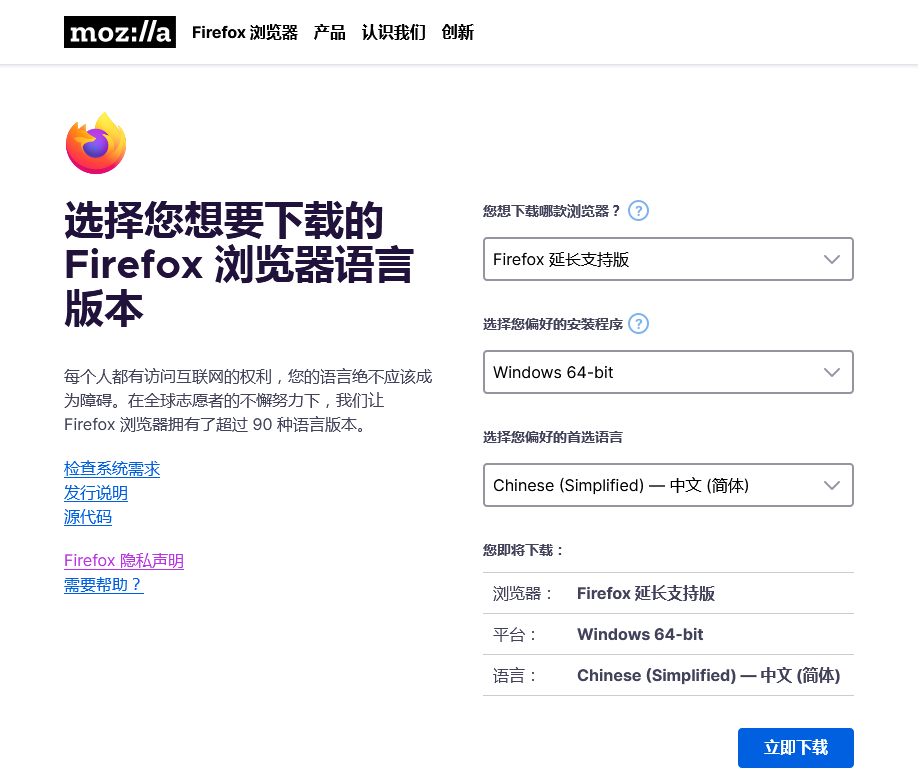
\includegraphics[width=5in]{media/image2.png}

接下来的教程使用延长支持版作为示例, 不同版本的浏览器在操作上存在些许差异, 如果您发现有不同之处, 请寻找有相近功能的按钮/入口. 

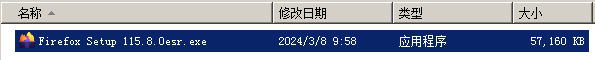
\includegraphics[width=5in]{media/image3.png}

作为访问互联网的入口, 浏览器可以为您提供大部分的功能, 双击运行上图所示的安装程序以开始安装. 

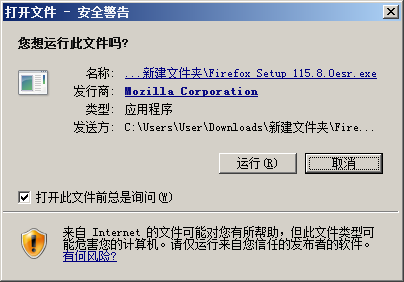
\includegraphics[width=2.5in]{media/image4.png}
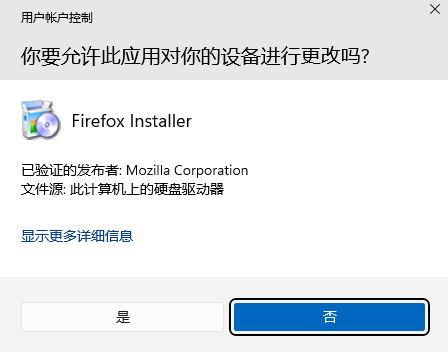
\includegraphics[width=2.5in]{media/windows-uac-dialog-win11.png} \\
这两个界面都是为了保护您的电脑不受病毒侵扰, 特此向您确认是否要继续. 请按【运行】或【是】. 

\newpage

接下来的安装界面如图所示: \\
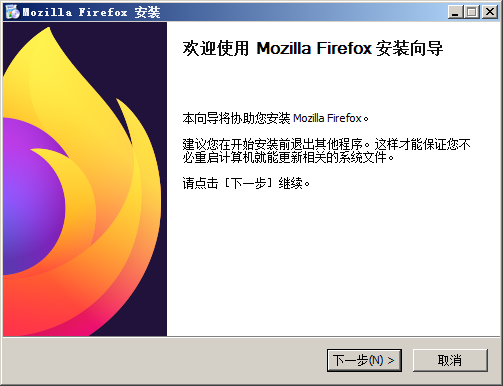
\includegraphics[width=2.5in]{media/image5.png}
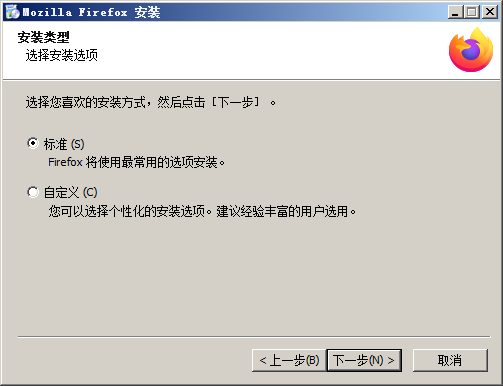
\includegraphics[width=2.5in]{media/image6.png} \\
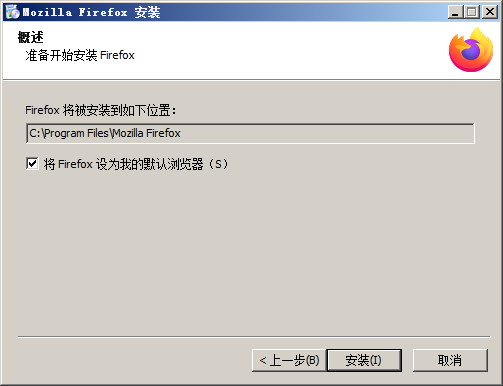
\includegraphics[width=2.5in]{media/image7.png}
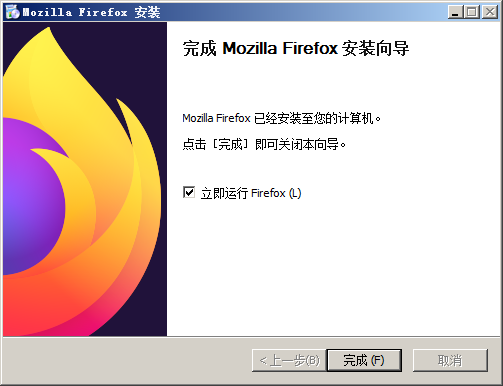
\includegraphics[width=2.5in]{media/image8.png}

运行Firefox后您会看到此界面: \\
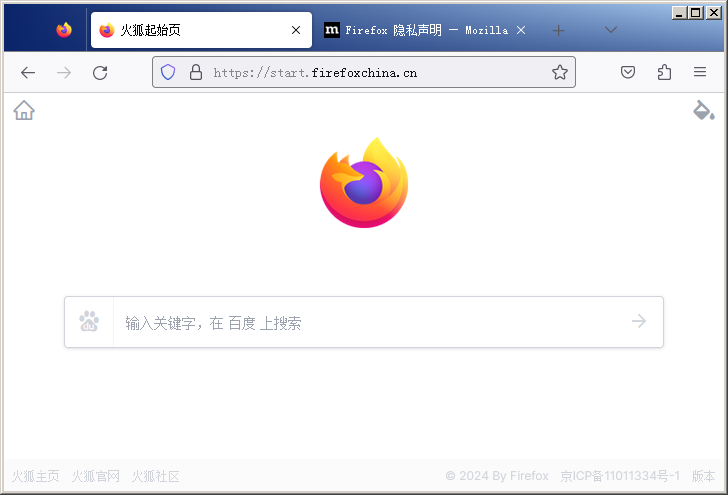
\includegraphics[width=5in]{media/image9.png}

单击地址栏 (或按下Ctrl+L组合键) , 这样您的键盘就开始待命, 准备接受输入, 尝试在地址栏键入一个网址, 例如: \url{baidu.com} \\
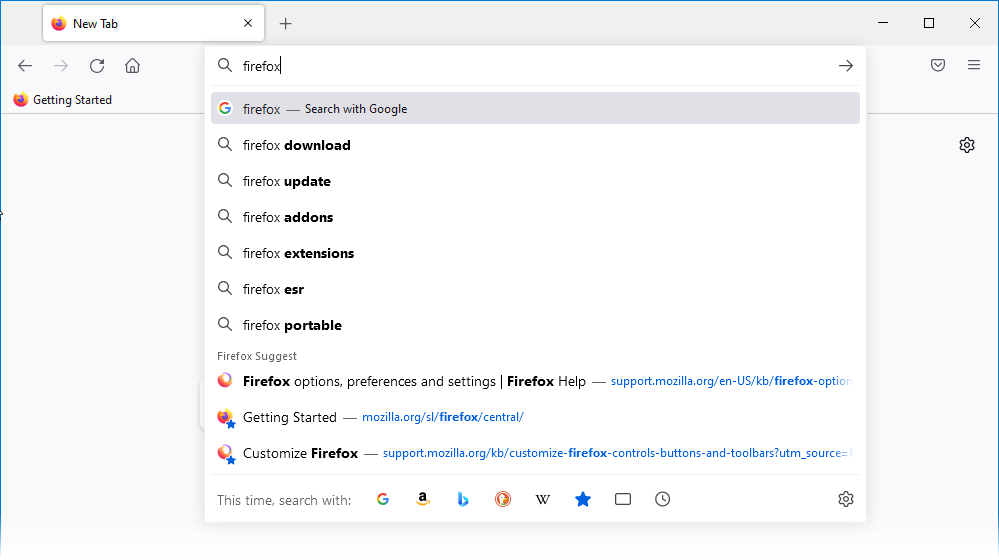
\includegraphics[width=5in]{media/44622-Fx96 Address bar autocomplete.png} \\
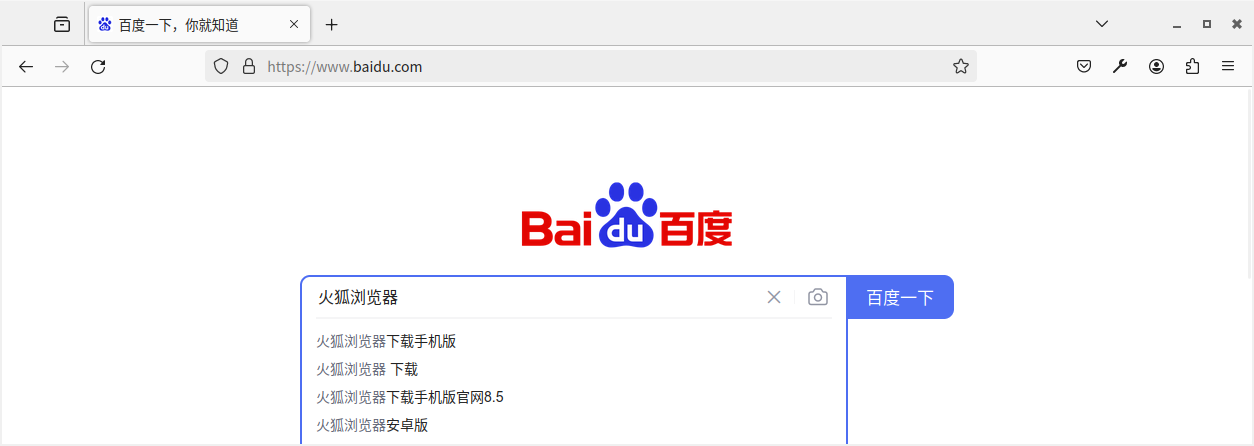
\includegraphics[width=5in]{media/firefox-search-baidu.png}

此外, 现代浏览器设计整合了地址栏与搜索栏的功能, 您亦可以在地址栏直接输入要搜索的内容, 然后按回车开始搜索. 

\subsection{网址}

您刚刚键入的 \url{baidu.com} 现在在地址栏中显示为 \url{http://www.baidu.com/}, 似乎有些不太一样, 但无伤大雅------因为网页如期打开了. 

这串网址, 专业术语叫URL (Uniform Resource Locator, 统一资源定位符) , 平日里只使用简称是完全不会引起问题的. 

其中\verb|http|是\textit{传输协议}, \verb|www.baidu.com|叫作\textit{域名}, 尾部的\verb|/|叫作\textit{路径分隔符}. \footnote{此处的说明做了简化处理, 有关更详细的说明, 请参阅本手册后文的对应章节. 这项内容实在复杂, 以至于出现了不少文章专门就“当你按下回车时, 究竟发生了什么”这一问题做出解答, 您可以搜索关键词“URL 按下回车”. }

传输协议一般有: 
\begin{itemize}
    \item \verb|http| 最常用的网络传输协议, \verb|https|则是它的安全加密版本
    \item \verb|ftp| 常见于文件上传下载, 近年来少见了, 不过在公司学校内部有时还会使用
\end{itemize}

访问一个网站需要与它的服务器建立连接, 为此需要知道服务器在哪里\footnote{技术上这个地址被称为\textit{IP地址}. }, 然后您的电脑就能与服务器通讯. 问题在于, 这个地址从人类的视角来看是长这样的: \verb|114.5.1.4|. \\
为此, 就像您通过查阅号码簿找到一个人名对应的电话号码一样: 电脑接受一个域名, 例如\verb|www.baidu.com|, 然后有一本号码簿可供电脑查询对于的地址. \footnote{技术上这个流程叫作\textit{DNS解析}, 这个号码簿叫作\textit{DNS服务器}. DNS服务器不止一台, 解析时, 电脑先查询根服务器, 然后查询com.服务器, 最后由baidu.com.服务器答复这个www.baidu.com.对应的IP地址. 这里域名结尾处多出的一点代表根服务器, 书写时省略, 电脑在处理时会自动补上, 但您看不到这个过程. }

您可能已经见过这样的URL: \url{https://github.com/yaii-project/yaii-manual} \\
它与前面那个的区别是, 后面带有一串\textit{路径}, 它指向 \verb|yaii-project| 文件夹下的  \verb|yaii-manual| 文件夹\footnote{技术上来说, 服务器会返回文件夹下的默认页面 (一般称为Index Page, 首页) . 值得一提的是, 早年间浏览器需要告诉服务器访问什么文件, 直接访问文件夹会出错, 现代服务器则会自动处理这种情况, 并返回Index Page. 浏览器方面不需要做任何处理, 就像它现在依旧访问的是一个普通文件一样. }

\section{关于本手册}

\subsection{获取本手册的最新版本}

由于您阅览的文件可能并非最新版本------这意味着有些东西会在未来失效------因此您应该考虑访问本手册的网页版本: \url{https://yaii-project.github.io/yaii-manual/zh}

\subsection{为本手册做出贡献}

当您也积累足够的知识之后, 您可以考虑为本手册做出贡献. 本手册的源代码托管于 \url{https://github.com/yaii-project/yaii-manual}

\endinput
